\chapter{Oblique Splits via Probabilistic Models}
\label{ObliqueSplitsviaProbabilisticModels}
This chapter presents a new approach to growing full oblique trees. The question of how one obtains interpretable oblique trees is deferred to Chapter~\ref{InterpretableObliqueTrees}.\\

This chapter is organised as follows. Section~\ref{IdealOutcomes} revisits original ideas behind tree growth which show how natural steps can be taken to find a small yet comprehensive set of oblique splits. As with indirect search approaches, the best split over this subset can be found upon which tree growth continues as usual. By identifying and solving a family of two-class classification problems similar to that of Brown \emph{et al} with linear classifiers, an interesting family of oblique splits is easily found. Section~\ref{RealizingObliqueSplits} discusses why logistic regression is chosen for this task. Section~\ref{ExamplesofObliqueTrees} demonstrates of this approach by growing oblique trees on several widely used classification datasets. This chapter concludes with a heuristic argument for the suitability of the subset considered.

\section{Ideal Outcomes}
\label{IdealOutcomes}
Existing approaches to tree growth find the split that minimizes impurity over some subset of the oblique split dictionary. Rather than jumping straight into this problem let us recall why splits with low impurity are desirable in the first place. \\

As mentioned in Section~\ref{ClassificationTrees}, a classification tree seeks to recursively partition observations into smaller subsets where observations have more similar classes. \emph{Node impurity} is a measure that quantifies this idea of class similarity at a node which according to Breiman \emph{et al}~\cite{cart84-2}(p. 24) should be zero when observed class probabilities are concentrated on one class and maximal when uniformly distributed over all classes. \emph{Split impurity} extends this idea of node impurity and quantifies the ability of a split to partition observations defined to be the weighted average impurity over child nodes resulting from such a split over the training set. In summary, split impurity is simply a proxy for the ability of a split to separate observations of different classes. \\

What are the ideal outcomes of a test at a node? Observations of different classes would be perfectly partition from each other, these are \emph{ideal outcomes}. There are many ways this could happen, with $R$ residual classes at a node there are in fact $2^{R-1}-1$ ideal outcomes (there are $2^{R-1}-1$ ways of binning $R$ balls into two non-empty buckets). To illustrate the idea of ideal outcomes, there are 7 ($=2^{4-1}-1$) ideal outcomes when there are 4 residual classes as listed in the titles of plots in Figure~\ref{fig:superclass1}.\\ 

\begin{figure}
\centering
\includegraphics*[width=.24\textwidth]{fig_superclass1_1.ps}
\includegraphics*[width=.24\textwidth]{fig_superclass1_2.ps}
\includegraphics*[width=.24\textwidth]{fig_superclass1_3.ps}
\includegraphics*[width=.24\textwidth]{fig_superclass1_4.ps}\\
\includegraphics*[width=.24\textwidth]{fig_superclass1_12.ps}
\includegraphics*[width=.24\textwidth]{fig_superclass1_13.ps}
\includegraphics*[width=.24\textwidth]{fig_superclass1_14.ps}
\caption{Ideal outcomes when there are 4 residual classes}
\label{fig:superclass1}
\end{figure}

For example, ideal outcome \{1\}\{2,3,4\} denotes the outcome of a test that perfectly separates all observations of class 1 from those of class 2, 3 and 4. Ideal outcomes are interesting targets to aim for as they exactly what one wishes to achieve during tree growth, it produces pure nodes quickly. \\

By considering ideal outcomes as two-class classification problems, these classification problems can be solved with linear classifiers to produce linear decision boundaries that approximately produce these ideal outcomes. As linear decision boundaries are synonymous with oblique splits, this process effectively produces oblique splits that partition observations of different classes (as demonstrated in Figure~\ref{fig:superclass1}). It is easy to see that ideal splits replicate ideal outcomes rather well in this example. Ideal split \{1\}\{2,3,4\} partitions most class 1 observations from other classes as do ideal splits \{3\}\{1,2,4\}, \{4\}\{1,2,3\}, \{1,3\}\{2,4\} and \{1,2\}\{3,4\}. Some ideal outcomes are not easily reproducible with oblique splits as shown by ideal split \{2\}\{1,3,4\} and \{1,4\}\{2,3\}. \\

As ideal splits are based on ideal outcomes which perfectly partition observations they should partition observations well and thus have low impurity values. As such, a family of $2^{R-1}-1$ oblique splits can be found when there are $R$ residual classes at a node.

\section{Realizing Oblique Splits}
\label{RealizingObliqueSplits}
There is a choice of which linear classifier is used to solve these two-class classification problems. Other than being linear additional qualities are desirable for such a classifier. These include,
\begin{description}
\item[Computationally light:] $2^{R-1}-1$ problems must be solved at each node so the cost of training such a classifier is greatly magnified by tree growth.
\item[Automated training:] Needing to solve so many problems, such a classifier should require minimal human input (if any at all). 
\item[Able to find separating hyperplanes:] Where two-class problems are linearly separable\footnote{Two-class classification data is linearly separable if there exists a hyperplane that partitions all observations of one class from the other} the classifier should find a separating hyperplane.
\item[Applicable to feature selection ideas:] Though unnecessary for the problem at hand, the ability to remove attributes to produce concise oblique splits is desirable.
\end{description}

With these criteria in mind we review several linear classifiers to see why logistic regression~\cite{cullagh-generalized} is used.

\begin{description}
\item[Perceptron Learners:] Perceptron learners do not converge in the presence of non-linearly separable data. %Utgoff \emph{et al} enforce convergence by using thermal perceptrons.
\item[Support Vector Machines:] Soft-margin support vector machines find ``separating hyperplanes'' with non-linearly separable data however a quadratic programming problem must be solved. In addition to this feature selection ideas do not seem to be applicable.
\item[Linear Discriminant Analysis:] Though straightforward to train, LDA does not always find separating hyperplanes on linearly separable data. 
\item[Linear Regression:] Feature selection techniques are applicable however linear regression does not always find separating hyperplanes on linearly separable data. 
\item[Logistic Regression:] Seeking to maximize a likelihood, logistic regression finds separating hyperplanes where one exists and feature selection ideas are applicable. Though numerical procedures for maximizing the likelihood may fail to converge, they can be overcome with simple checks and so they can be trained in an automated fashion. 
\end{description}
It is for these reasons that logistic regression is chosen for solving these two-class classification problems.\\

Upon fitting a binomial logistic regression model, the equation for the decision boundary must be extracted. This is straightforward. The binomial logistic regression model assumes the posterior log-odds of one class against the other (say the 2nd to the 1st) has the following form $$\log\frac{P(G=2|X=x)}{P(G=1|X=x)}=a+\sum_{i=1}^q a_i x_i.$$ As the decision boundary is located where the posterior odds of the two classes are equal it is simply where the log-odds equals zero, i.e. the equation of the oblique split found via logistic regression is given by the linear form with its maximum likelihood plug-in estimates $$\hat{a}+\sum_{i=1}^q \hat{a}_i x_i=0.$$ 

\section{Examples of Oblique Trees}
\label{ExamplesofObliqueTrees}
As mentioned in Section~\ref{SummaryofExistingWork}, one of the shortcomings of existing work is the unavailability of easily useable implementations. Ideas mentioned in this thesis are all implemented in R to address this issue and are used throughout this thesis to demonstrate ideas. \\

The function \texttt{oblique.tree(formula,data,subset,split.impurity,...)} allows various types of classification trees to be grown including,
\begin{enumerate}
\item Axis-parallel trees: that use axis-parallel splits exclusively\\
\texttt{oblique.tree(...,oblique.splits="off")}
\item Mixture trees: that consider both axis-parallel and oblique splits (whichever has the lowest impurity)\\
\texttt{oblique.tree(...,oblique.splits="on")}
\item Oblique trees: that use oblique splits exclusively\\
\texttt{oblique.tree(...,oblique.splits="only")}
\end{enumerate}
!!!!!!!!!!!!!!!!!!!
The exact stopping criteria of tree growth is as follows. Nodes are no longer partitioned if any of the following is true.
\begin{enumerate}
\item Pure nodes: if all observation are of the same class
\item Deviance threshold: if the deviance of a node is below some prespecified proportion of the deviance of the root node (defaulted to 0.01)
\item Size threshold: if the number of observations is less than some prespecified limit (defaulted to 10)
\item Child node threshold: if all splits result in a child node with less than some prespecified number of observations (defaulted to 5).
\end{enumerate}
!!!!!!!!!!!!!!!!!!!!!

As oblique splits are better able to partition observations, the above three trees should require progressively fewer tests in theory. All three are grown on several classification datasets with the same stopping criteria to allow fair comparison and no attempt is made to improve their interpretability.

\subsection{Original Crabs Data}
\label{OriginalCrabsData}
Starting with the crabs dataset, it consists of 5 morphological measurements of 200 crabs (50 crabs of two colours from both sexes) collected at Fremantle, W. Australia. As significant variation the data arises due to differing maturities of crabs, this dataset is often used to demonstrate the principal components analysis technique. Using this data, Figure~\ref{fig:oblique_splits_crabs_original} shows the above three trees are grown to this data. \\

\begin{figure}
\centering
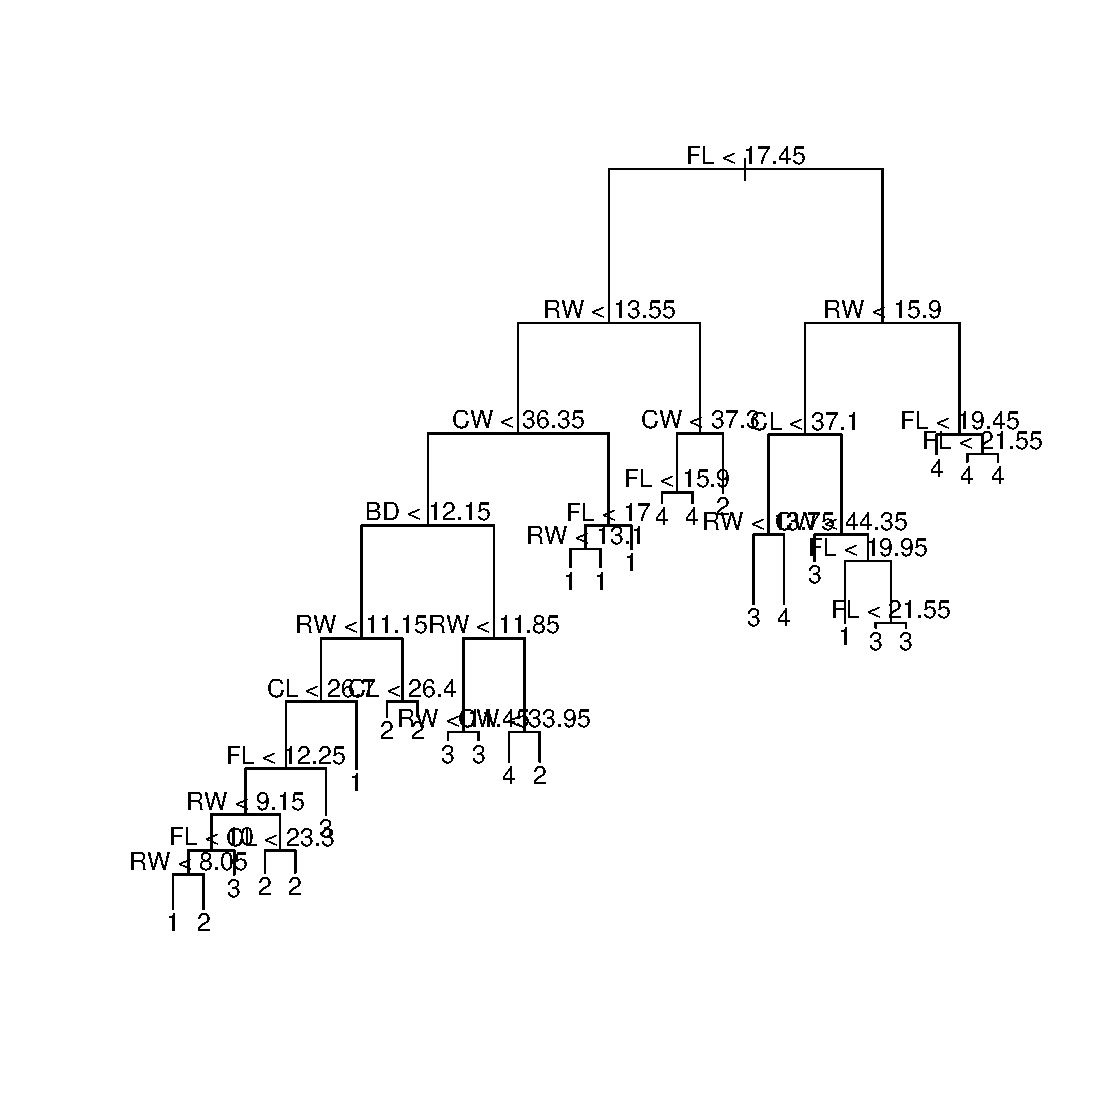
\includegraphics[width=.32\textwidth]{oblique_splits_crabs_original_off_tree.ps}
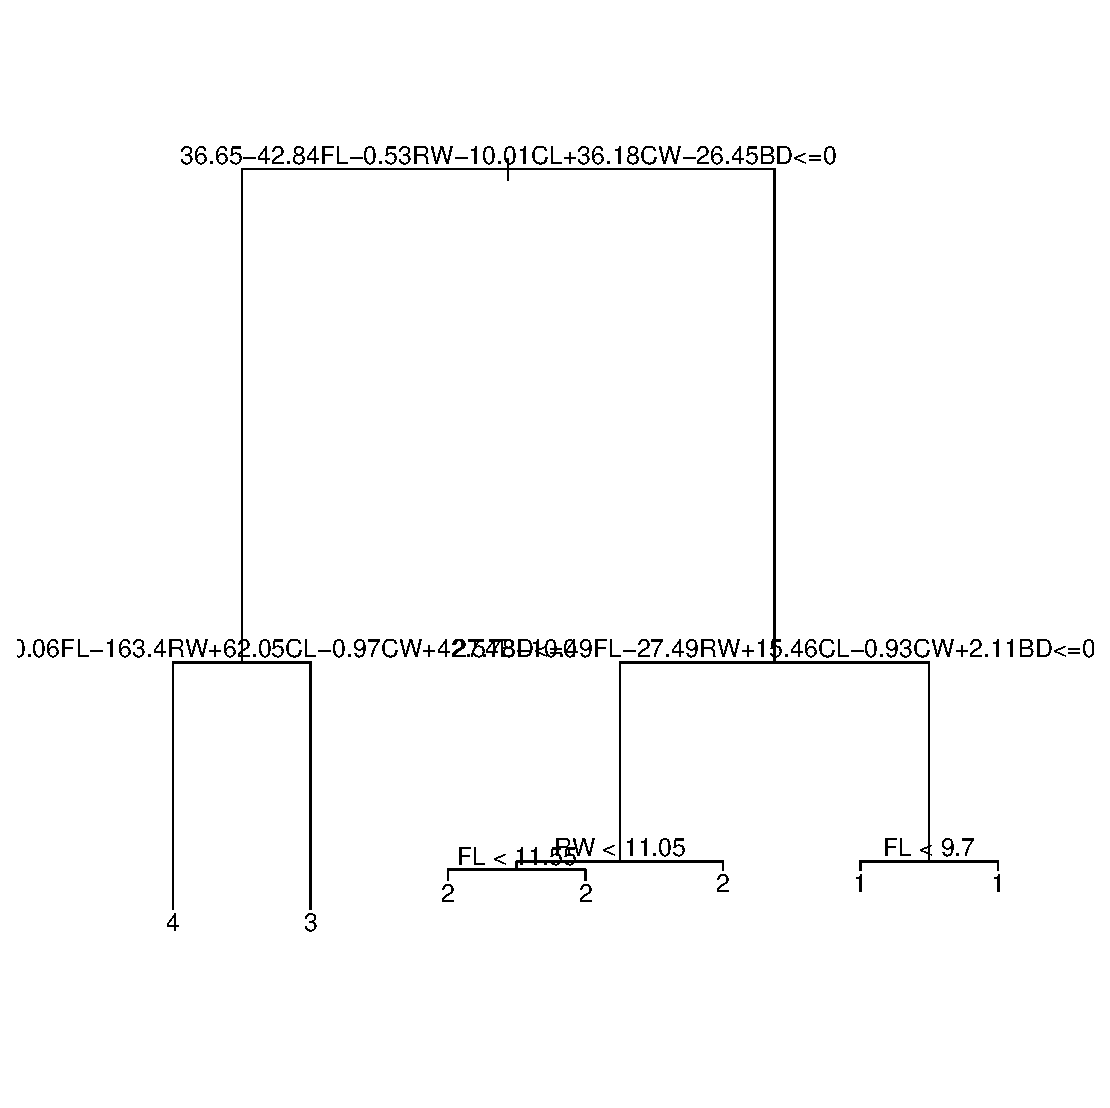
\includegraphics[width=.32\textwidth]{oblique_splits_crabs_original_on_tree.ps}
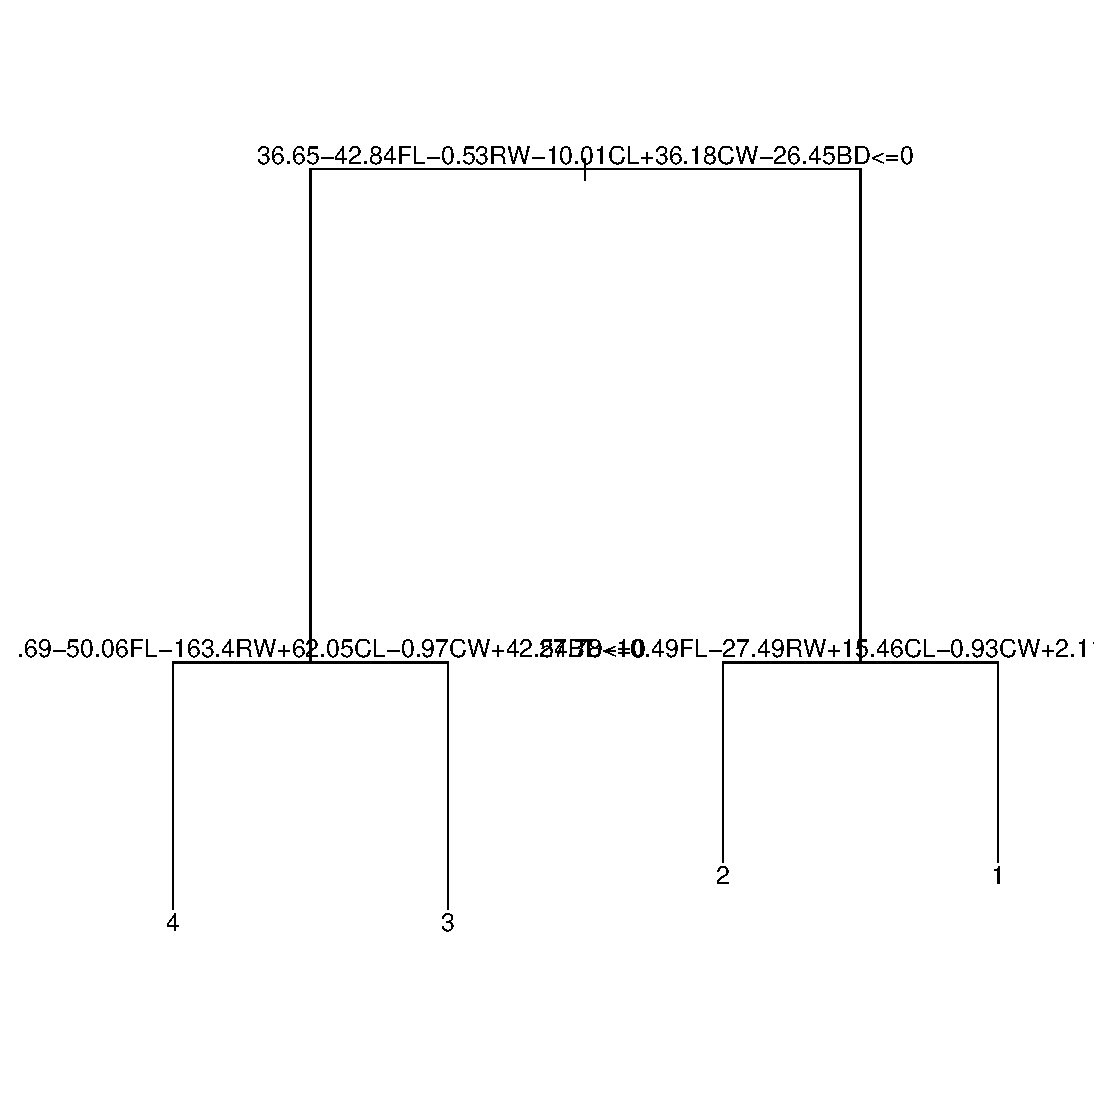
\includegraphics[width=.32\textwidth]{oblique_splits_crabs_original_only_tree.ps}
\caption{Axis-parallel tree, mixture tree and oblique tree grown on original crabs dataset}
\label{fig:oblique_splits_crabs_original}
\end{figure}

It is known that observations of different classes are well separated by oblique splits in this dataset. The axis-parallel tree grown is rather large as requires concatentated use of axis-parallel splits to partition observations. Allowing oblique splits, mixture trees and oblique trees use oblique splits to produce large reductions in deviance. \\

It should also be noted that when using oblique splits exclusively, only 7 (=$2^{4-1}-1$) splits need to be evaluated at the root node as compared to the 995 odd ($\approx(200-1)\times 5$) in the case of axis-parallel trees.

\subsection{Augmented Crabs Data}
\label{AugmentedCrabsData}
By projecting the crabs dataset onto its principal components second and third principal components, observations of different classes are much better separated. Axis-parallel trees should perform better on this \emph{Augmented Crabs dataset} as a result. With a 2-dimensional dataset, it is also possible to view the decision boundaries of each tree as is shown in Figures~\ref{fig:oblique_splits_crabs_augmented_off}-~\ref{fig:oblique_splits_crabs_augmented_only}.\\

\begin{figure}
\centering
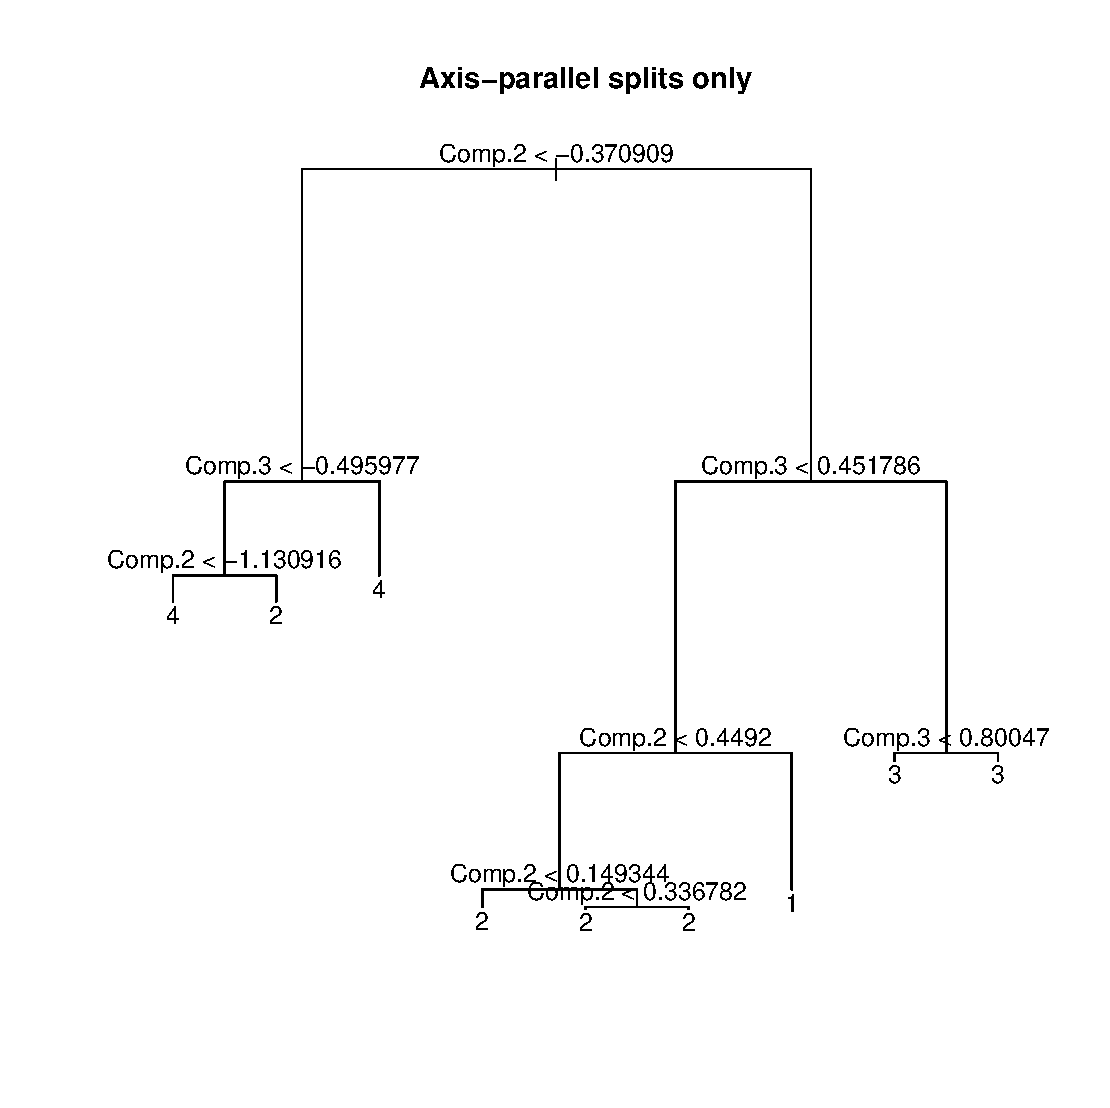
\includegraphics[width=.4\textwidth]{oblique_splits_crabs_augmented_off_tree.ps}
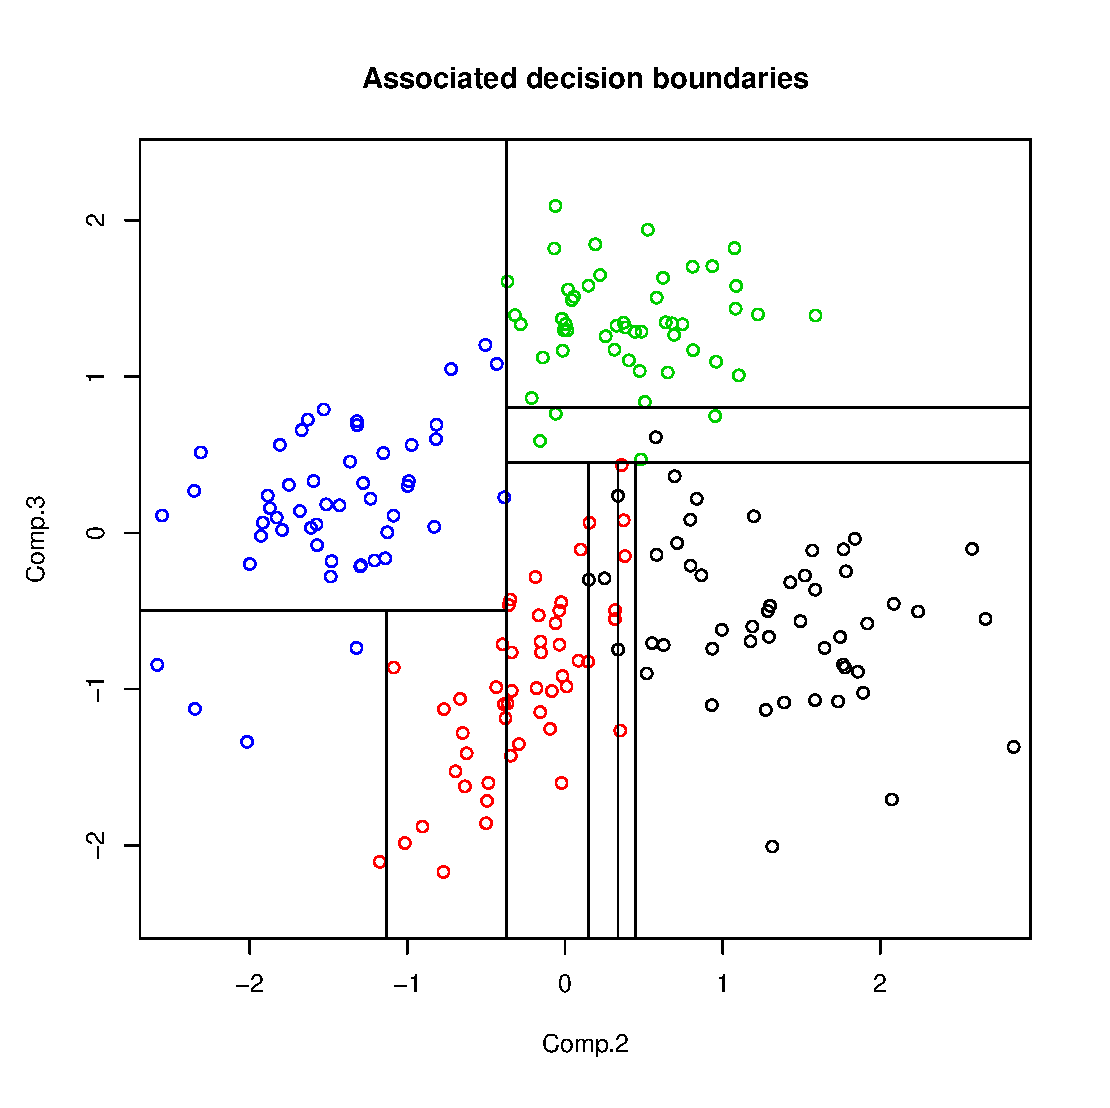
\includegraphics[width=.4\textwidth]{oblique_splits_crabs_augmented_off_decision_boundaries.ps}
\caption{Axis-parallel tree grown on the Augmented Crabs dataset with its associated decision boundaries}
\label{fig:oblique_splits_crabs_augmented_off}
\end{figure}
\begin{figure}
\centering
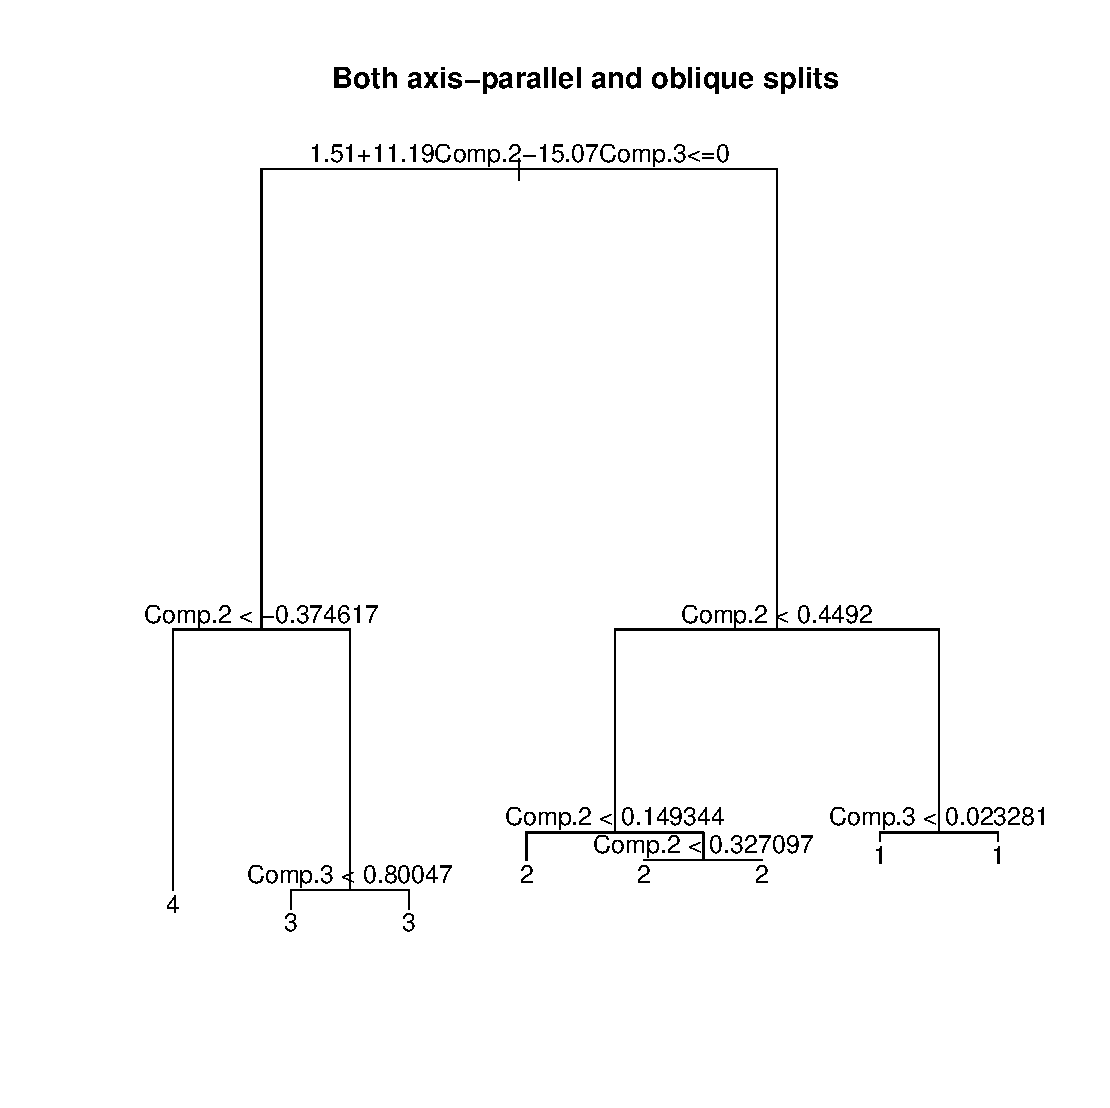
\includegraphics[width=.4\textwidth]{oblique_splits_crabs_augmented_on_tree.ps}
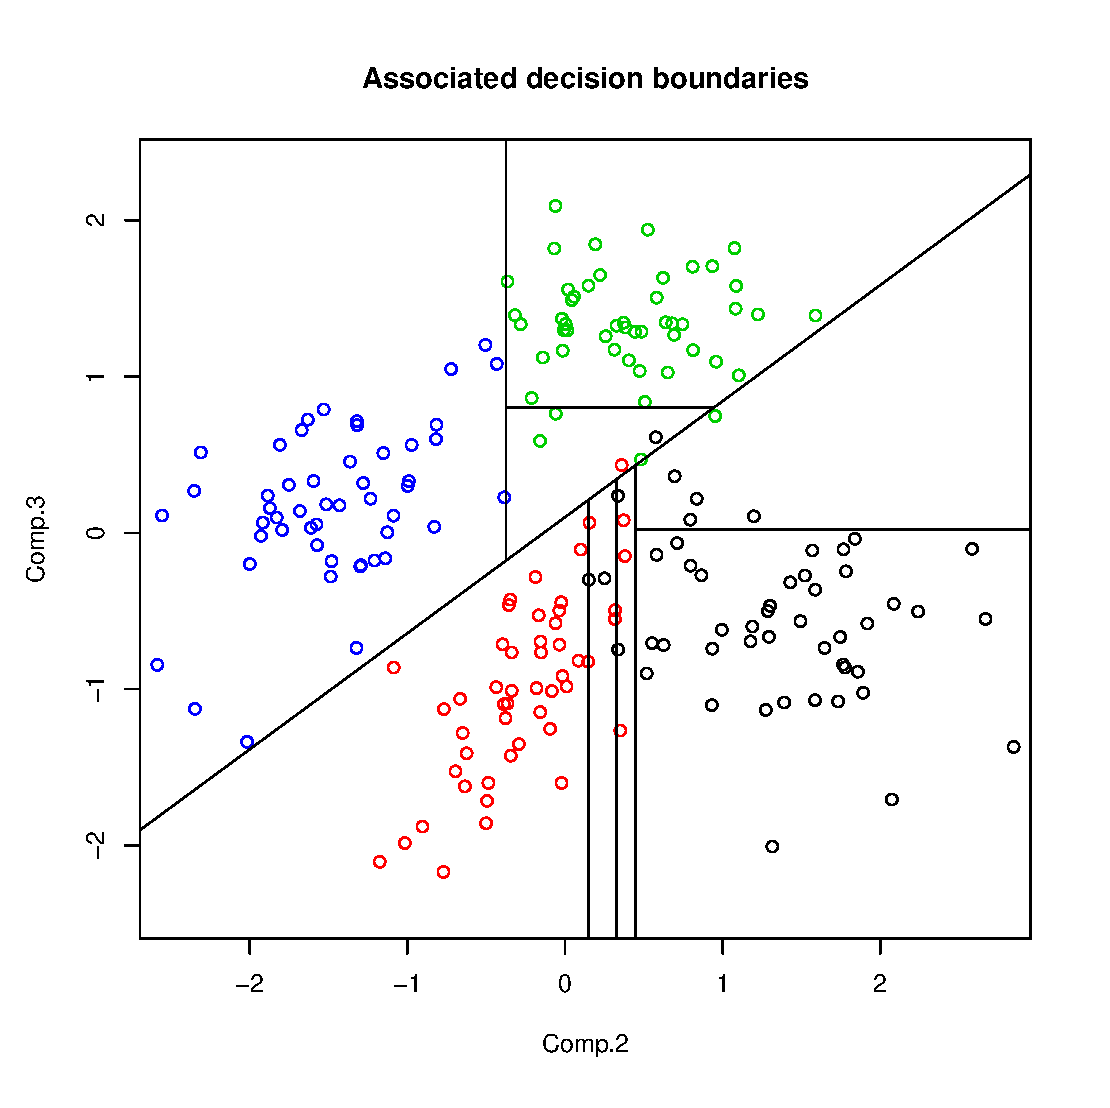
\includegraphics[width=.4\textwidth]{oblique_splits_crabs_augmented_on_decision_boundaries.ps}
\caption{Mixture tree grown on the Augmented Crabs dataset with its associated decision boundaries}
\label{fig:oblique_splits_crabs_augmented_on}
\end{figure}
\begin{figure}
\centering
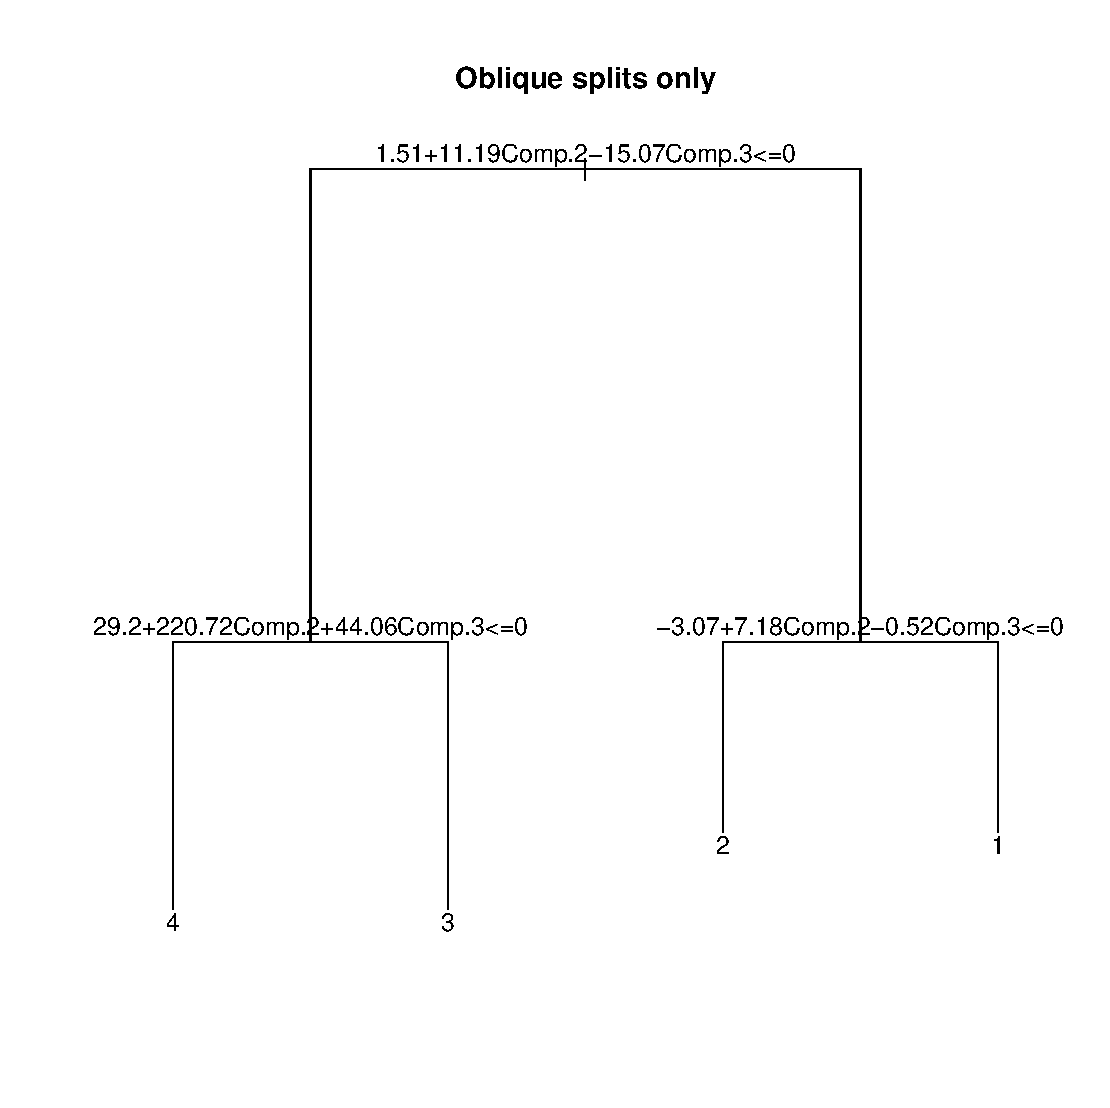
\includegraphics[width=.4\textwidth]{oblique_splits_crabs_augmented_only_tree.ps}
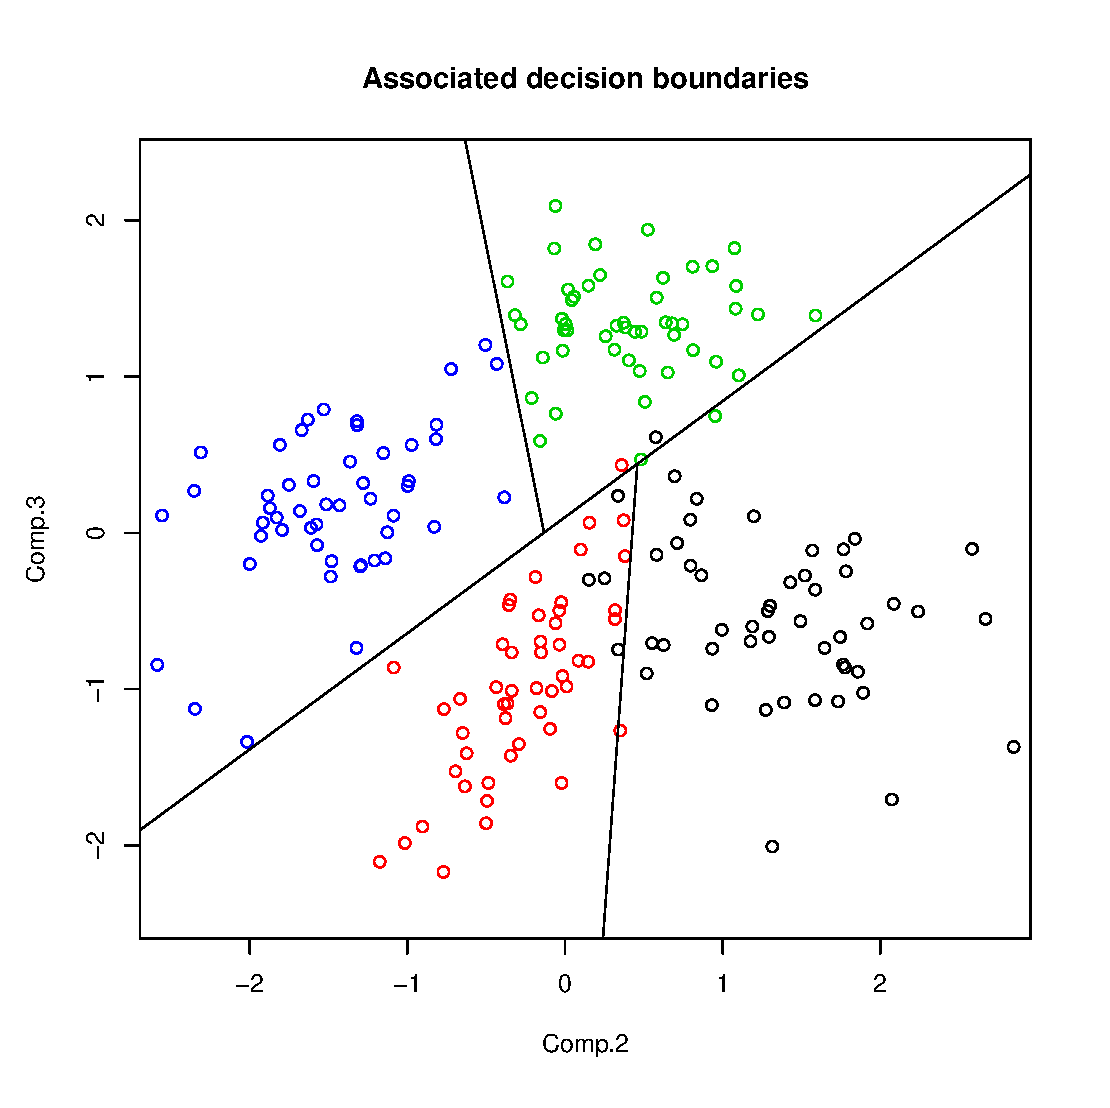
\includegraphics[width=.4\textwidth]{oblique_splits_crabs_augmented_only_decision_boundaries.ps}
\caption{Oblique tree grown on the Augmented Crabs dataset with its associated decision boundaries}
\label{fig:oblique_splits_crabs_augmented_only}
\end{figure}

Looking at the trees, the axis-parallel tree is indeed smaller than the one grown on the original crabs dataset however when compared to mixture and oblique trees, it still uses more tests. By examining decision boundaries of each tree, it is easy to see why. Observations are best partitioned with oblique splits.

\subsection{Pima Indians Data}
\label{PimaIndiansData}
The Pima Indians dataset contains 7 measurements from 532 women of Pima Indian heritage living near Pheonix, Arizona tested for the presence (or lackthereof) of diabetes. A subset containing 200 observations called \texttt{Pima.tr} found in the \emph{Modern Applied Statistics with S-Plus} library in R is used as the training set. Trees grown on this dataset are shown in Figure~\ref{fig:oblique_splits_pima_trees} both with and without text for greater clarity.\\

\begin{figure}
\centering
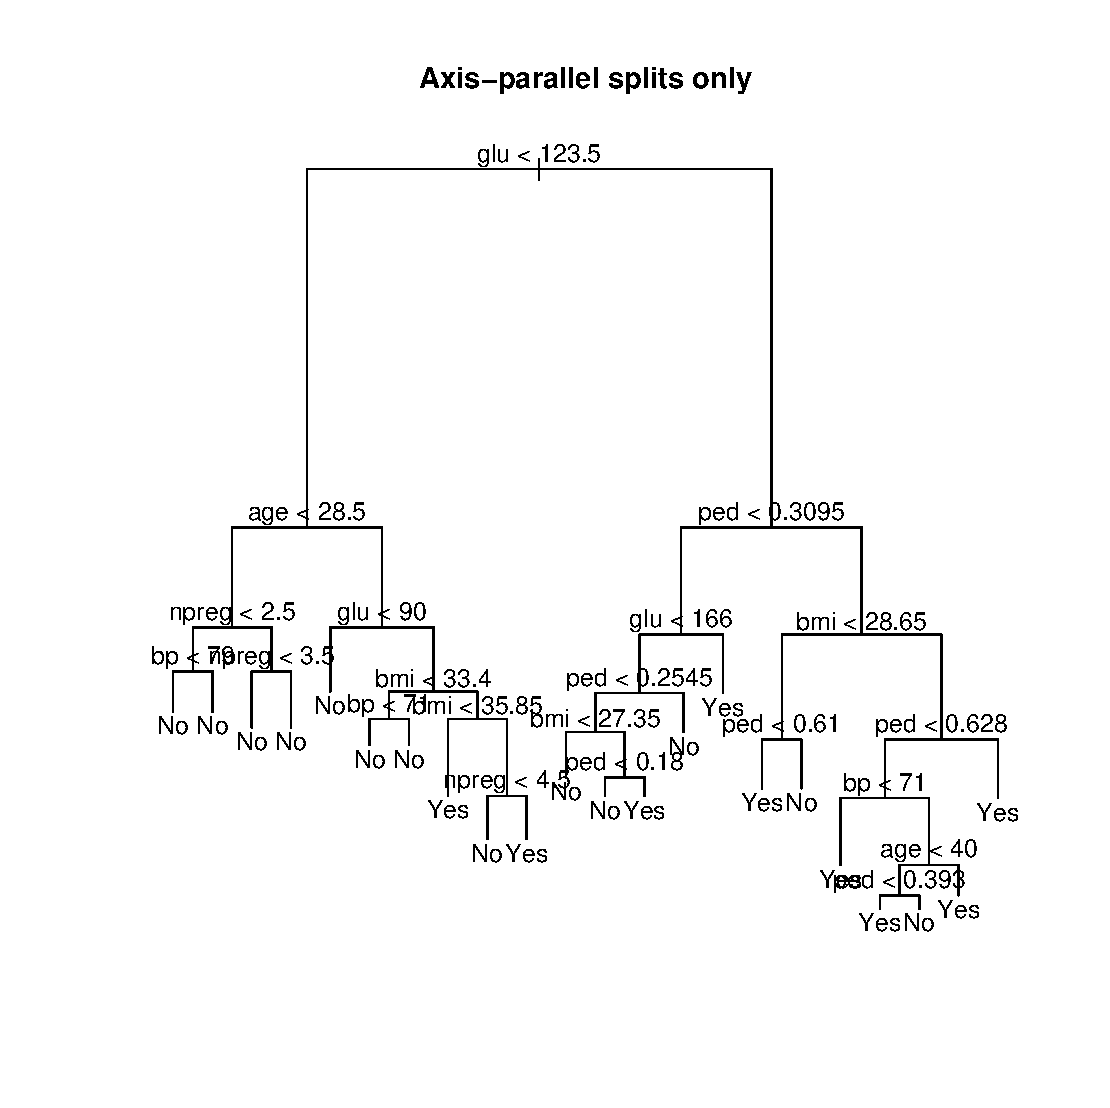
\includegraphics[width=.32\textwidth]{oblique_splits_pima_off_tree.ps}
\includegraphics[width=.32\textwidth]{oblique_splits_pima_on_tree.ps}
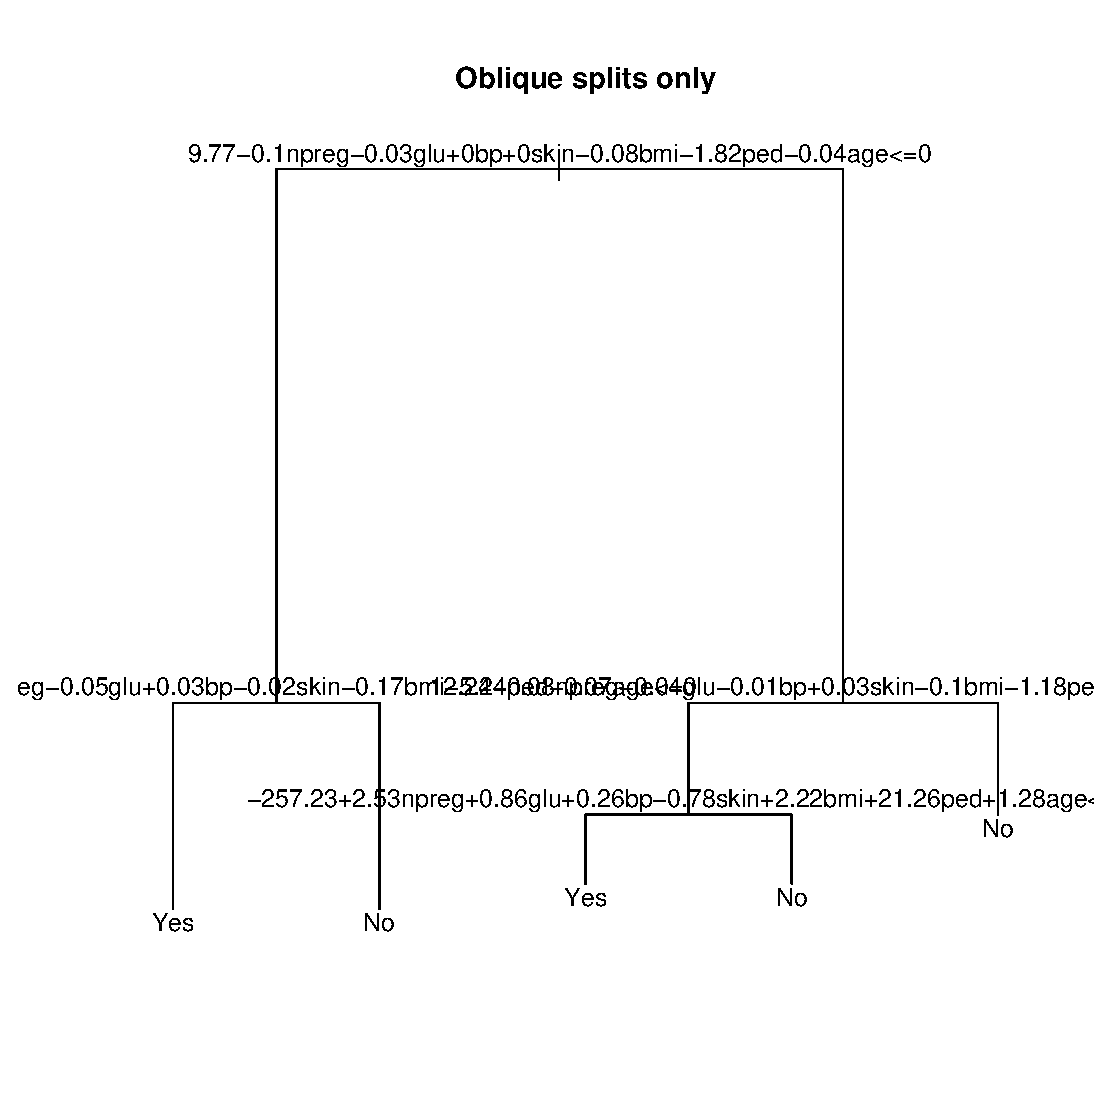
\includegraphics[width=.32\textwidth]{oblique_splits_pima_only_tree.ps}\\
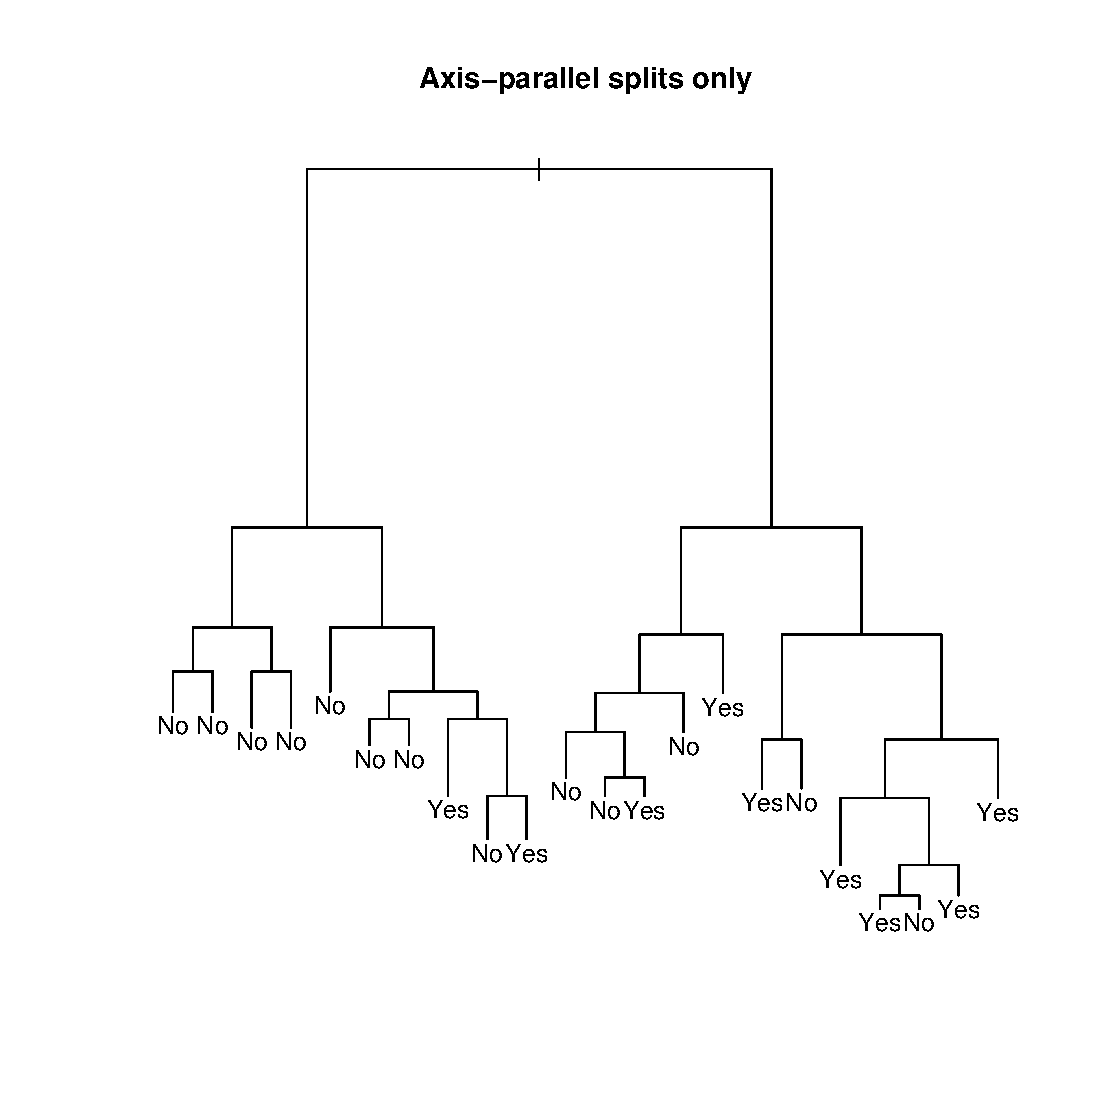
\includegraphics[width=.32\textwidth]{oblique_splits_pima_off_tree_skeleton.ps}
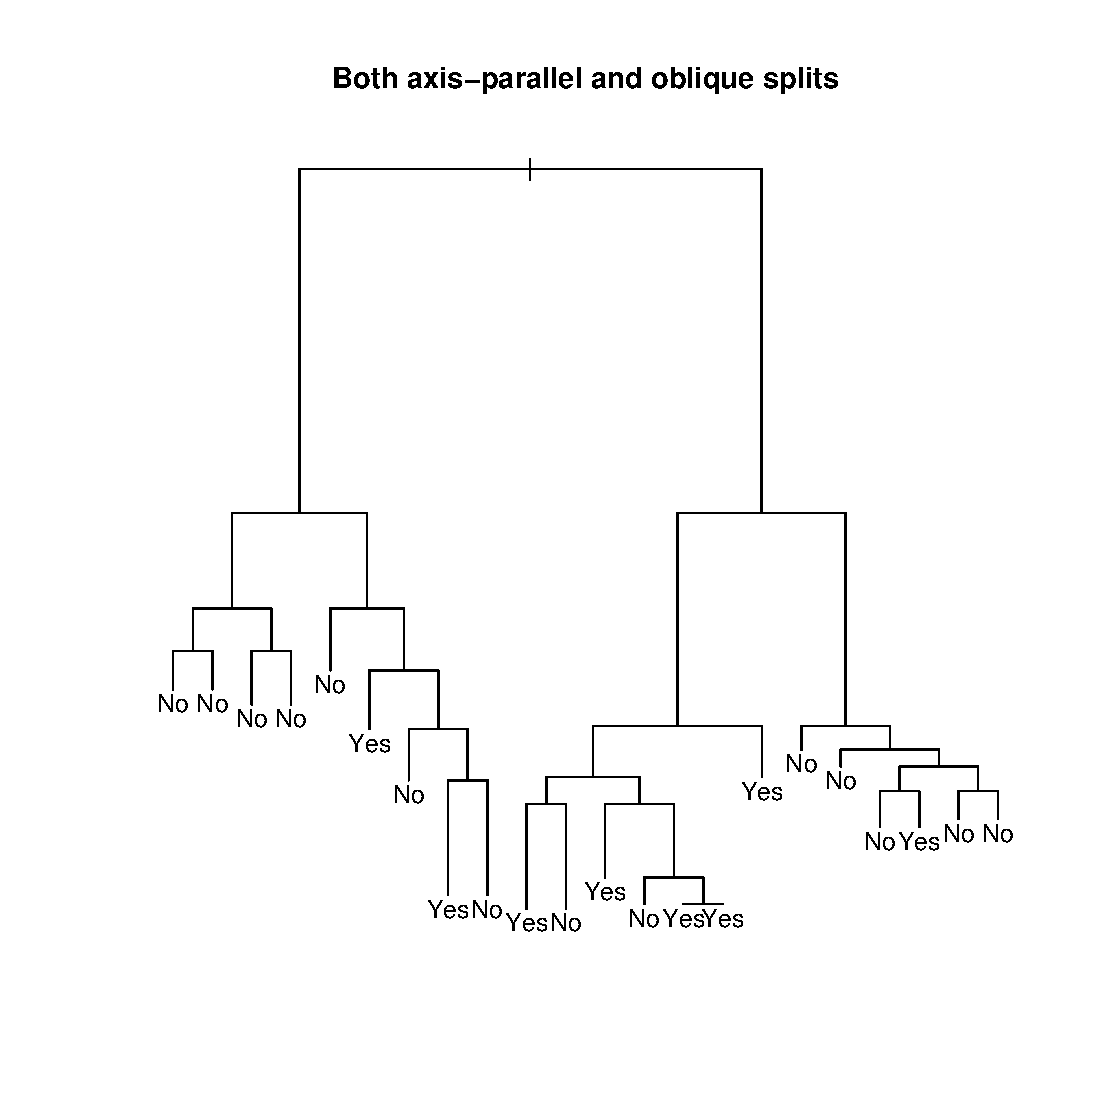
\includegraphics[width=.32\textwidth]{oblique_splits_pima_on_tree_skeleton.ps}
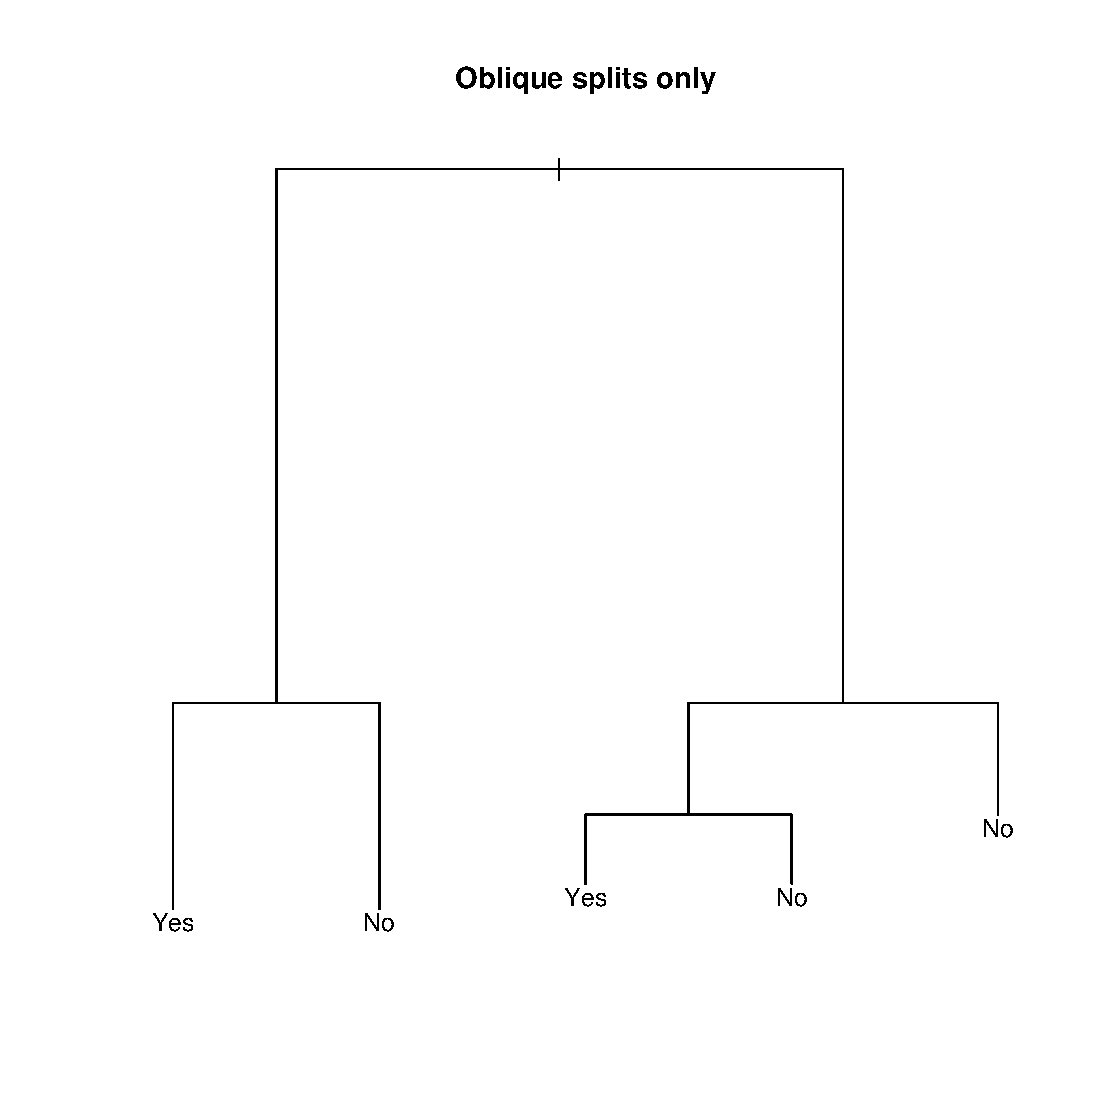
\includegraphics[width=.32\textwidth]{oblique_splits_pima_only_tree_skeleton.ps}
\caption{Trees grown on the Pima Indians dataset and their associated tree skeletons}
\label{fig:oblique_splits_pima_trees}
\end{figure}

As with before, much few tests are used when oblique splits are used.\\

\subsection{Glass Fragments Data}
\label{GlassFragmentsData}
The same can be said for the Glass Fragments dataset.
\begin{figure}
\centering
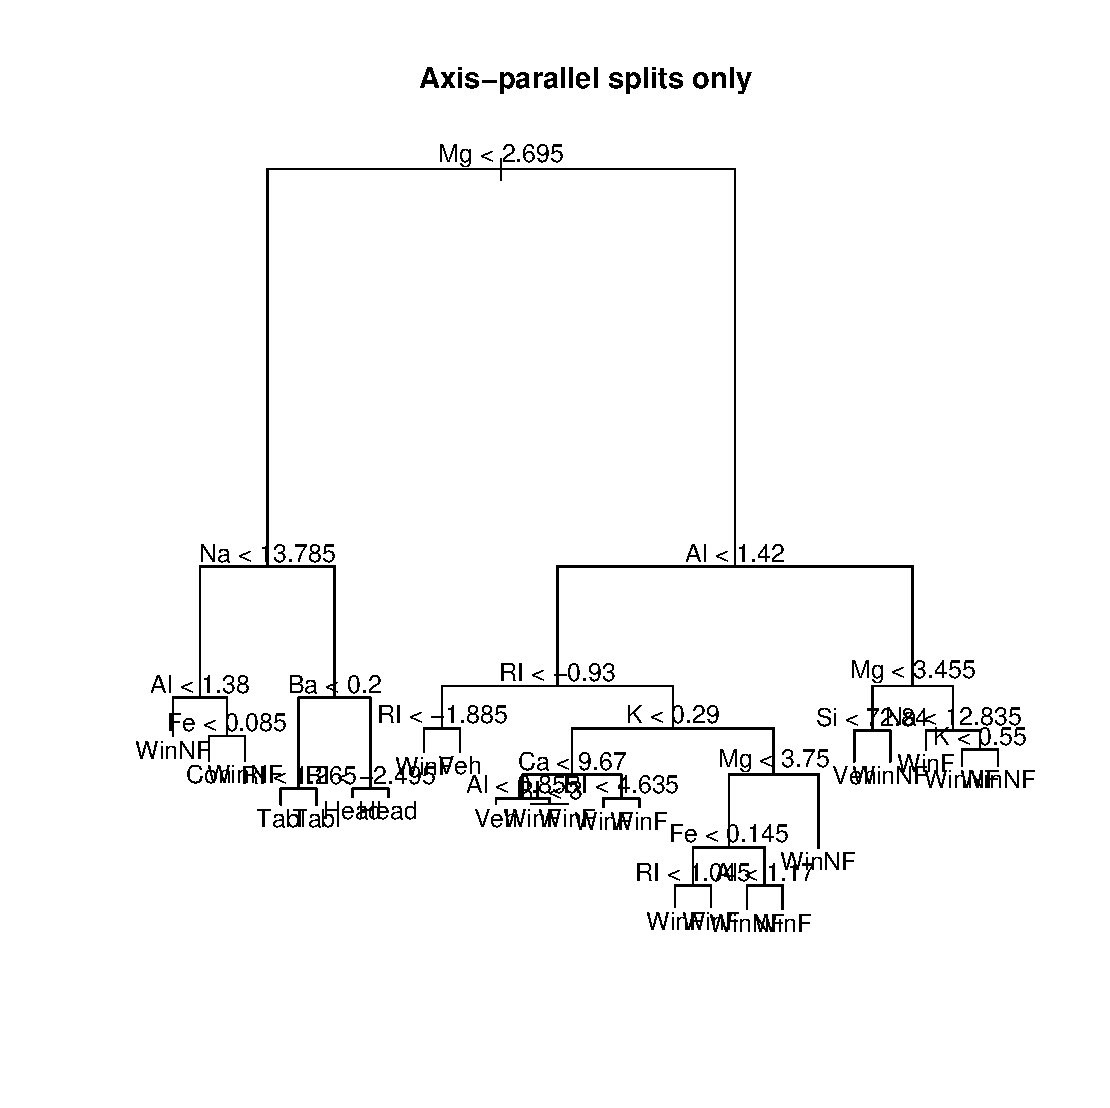
\includegraphics[width=.32\textwidth]{oblique_splits_fgl_off_tree.ps}
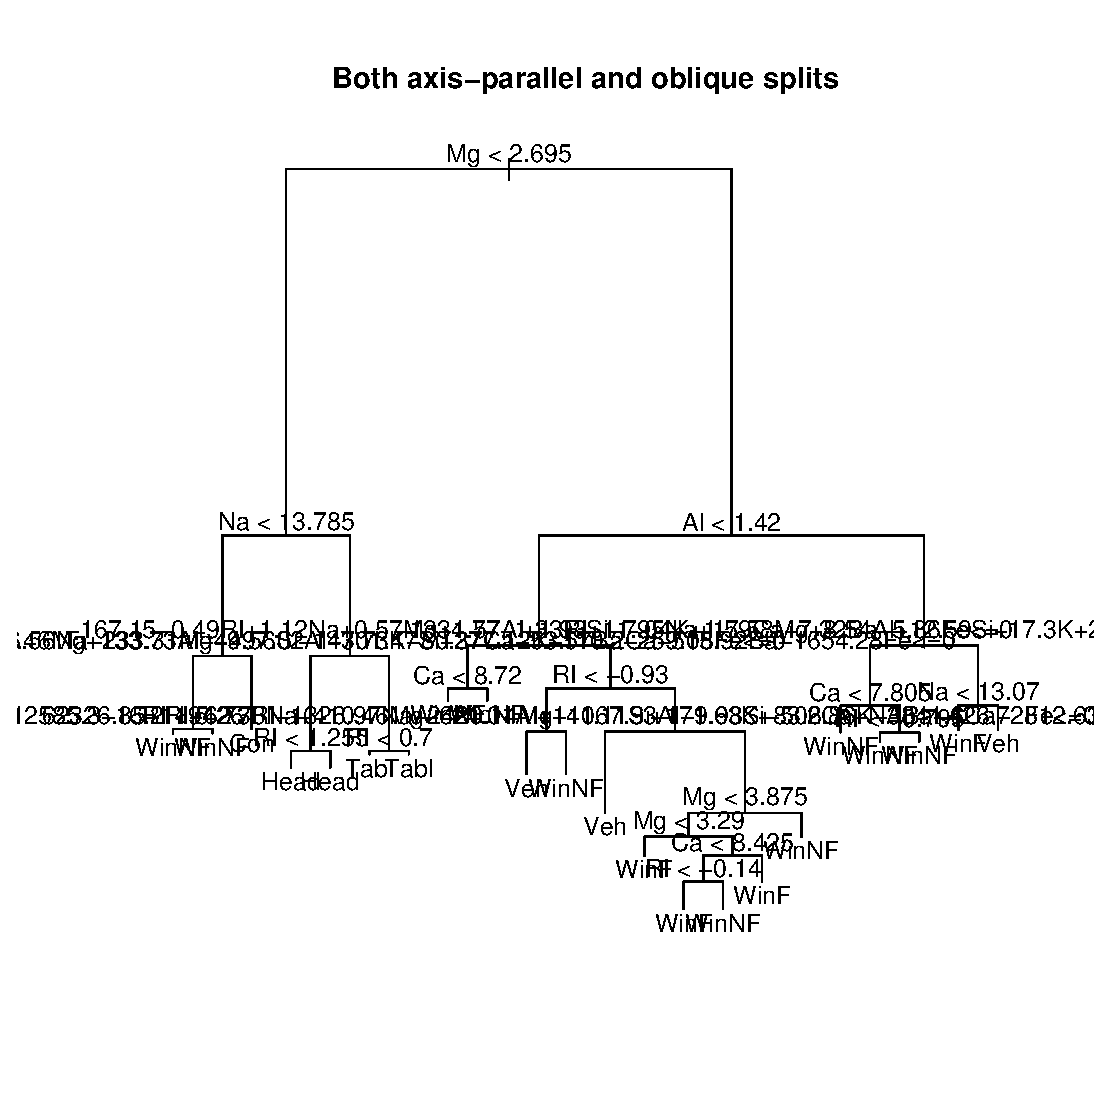
\includegraphics[width=.32\textwidth]{oblique_splits_fgl_on_tree.ps}
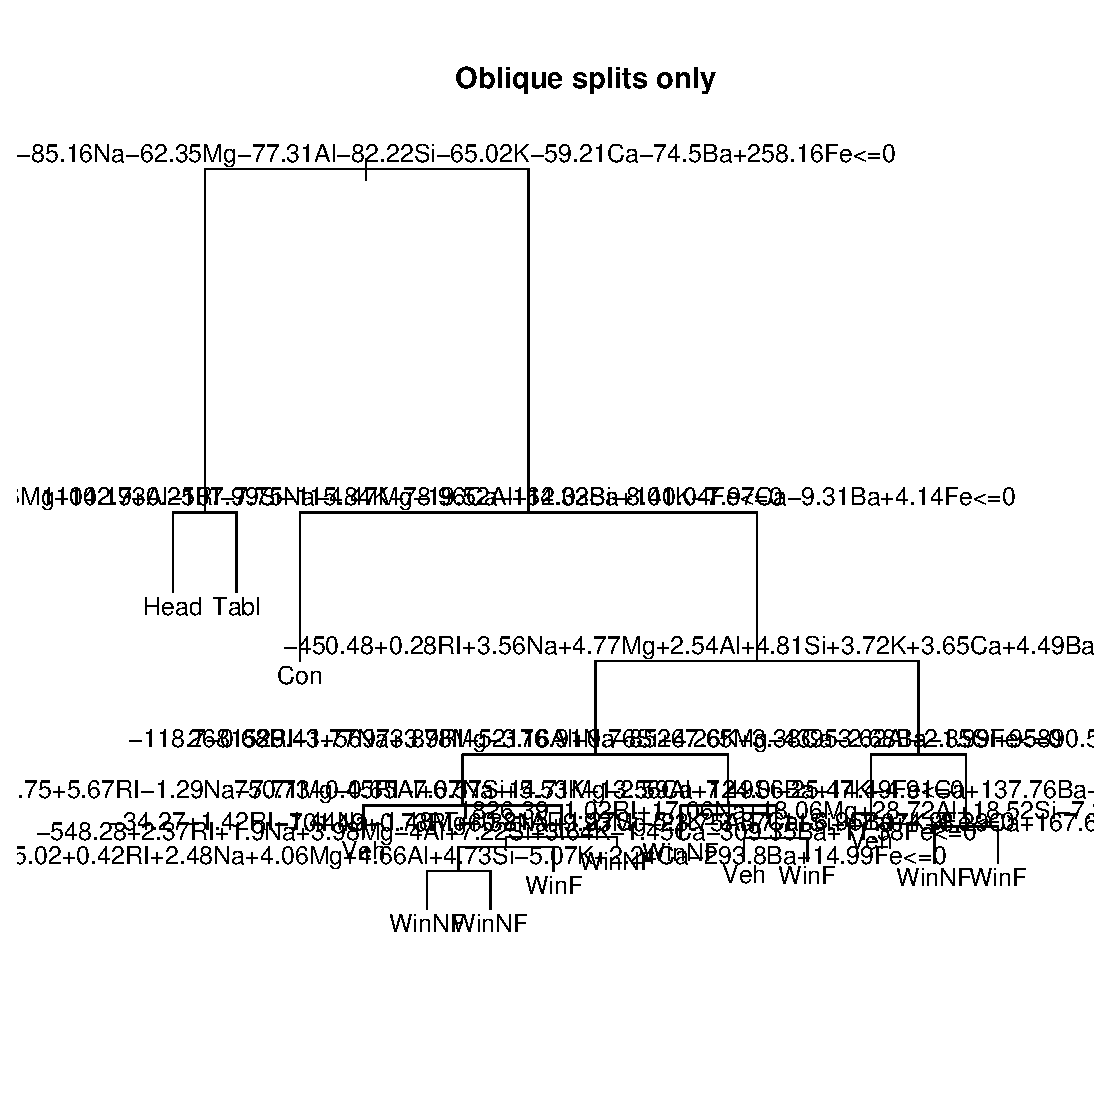
\includegraphics[width=.32\textwidth]{oblique_splits_fgl_only_tree.ps}\\
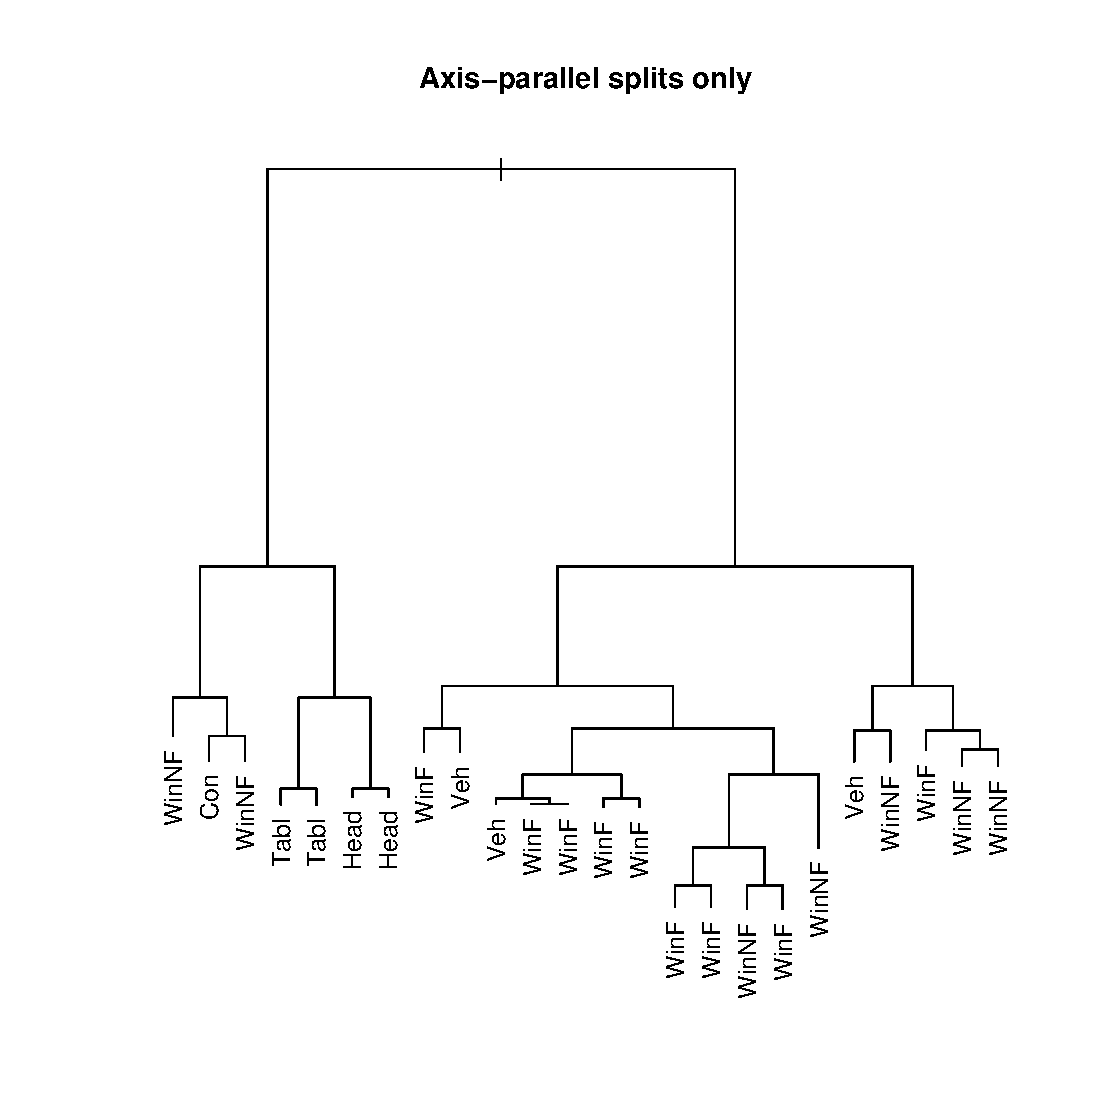
\includegraphics[width=.32\textwidth]{oblique_splits_fgl_off_tree_skeleton.ps}
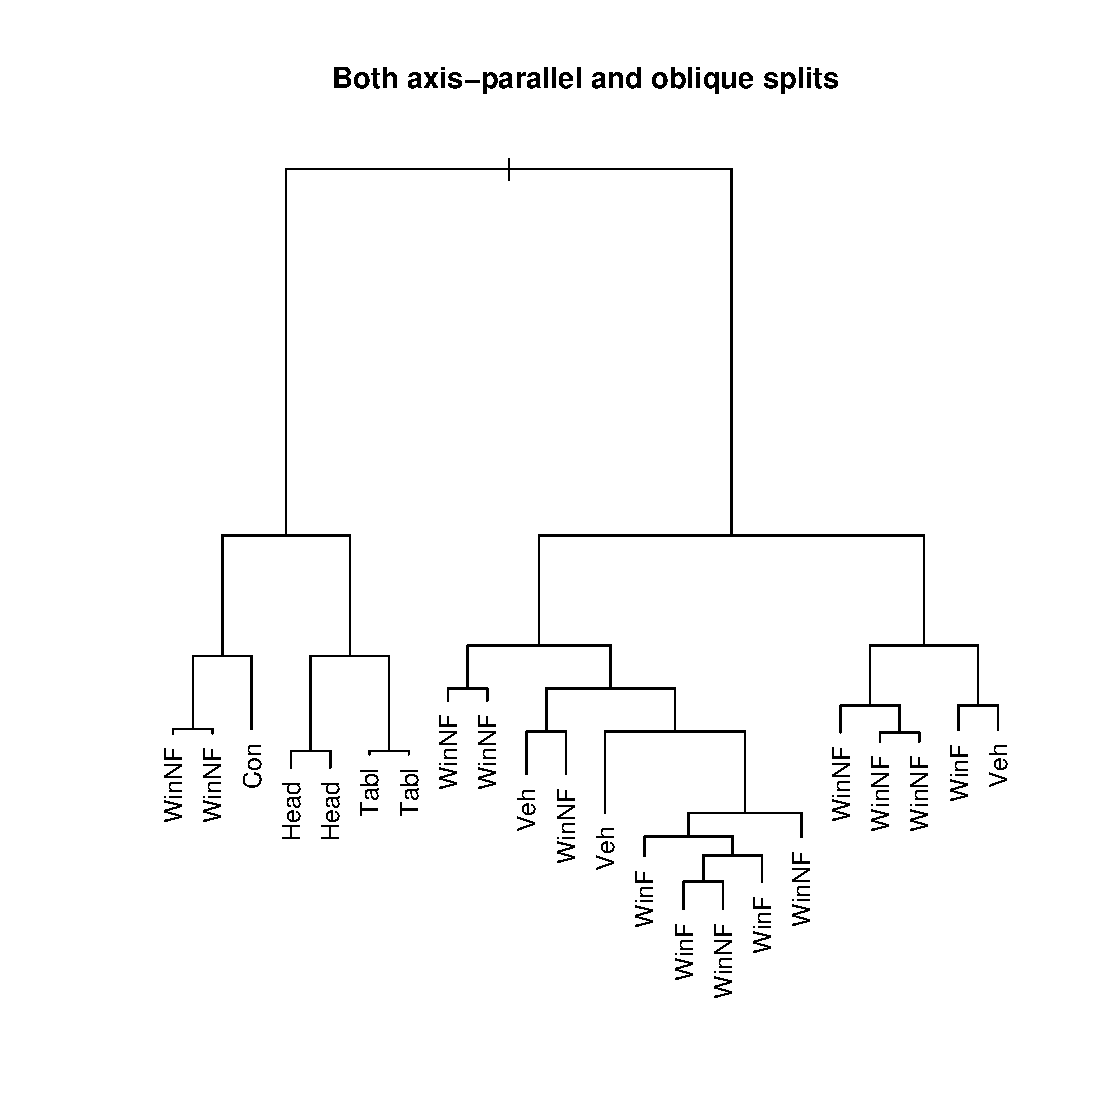
\includegraphics[width=.32\textwidth]{oblique_splits_fgl_on_tree_skeleton.ps}
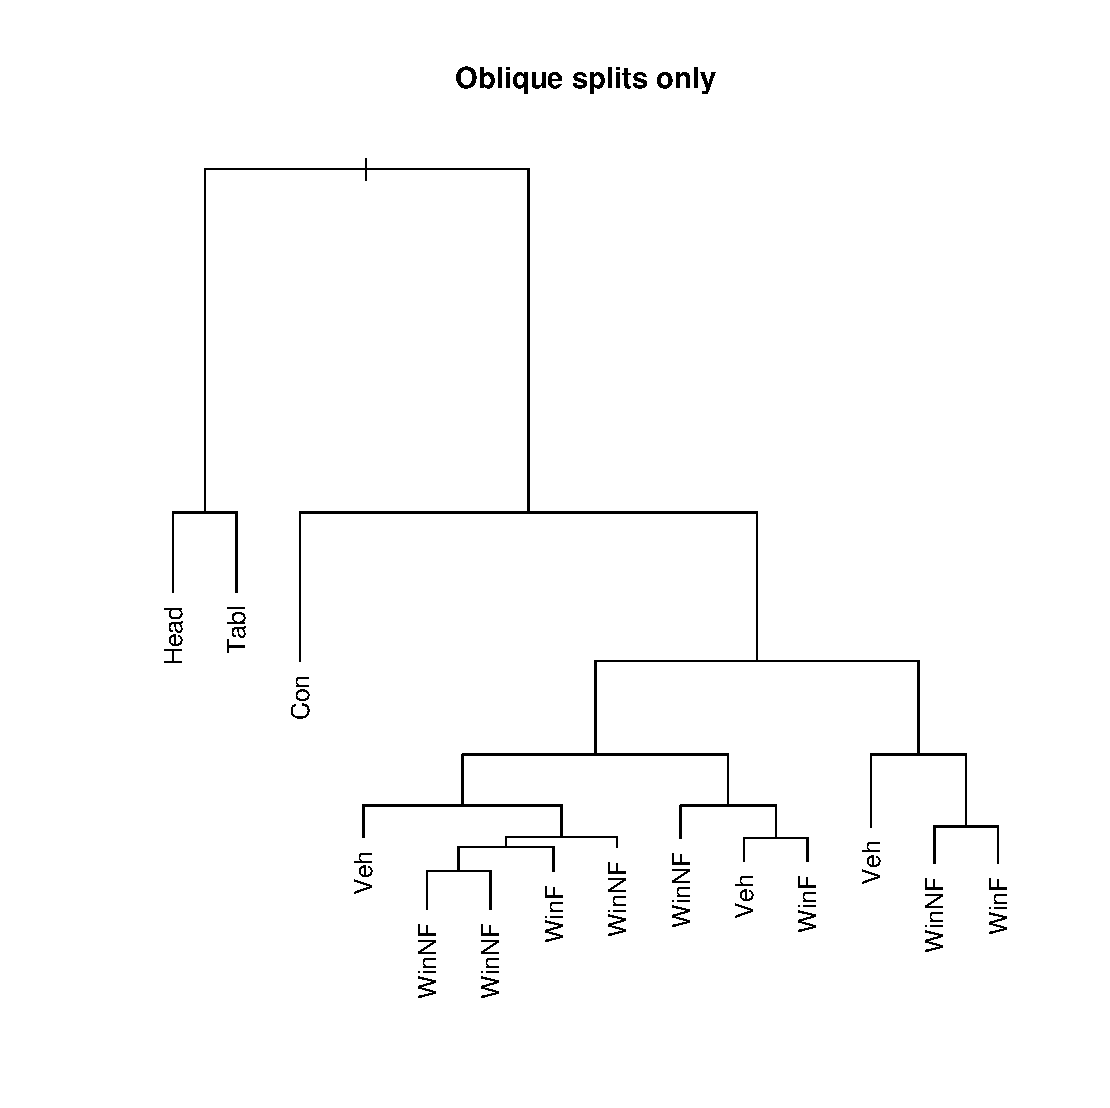
\includegraphics[width=.32\textwidth]{oblique_splits_fgl_only_tree_skeleton.ps}
\caption{Trees grown on the Glass Fragments dataset and their associated tree skeletons}
\label{fig:oblique_splits_fgl_tree}
\end{figure}

\section{Locally Optimal Subset}
\label{LocallyOptimalSubset}
The family of oblique splits specified in Section~\ref{IdealOutcomes} is intuitively appealing and as Section~\ref{ExamplesofObliqueTrees} shows allows interesting oblique trees to be grown. With an oblique split dictionary of size $\sum_{k=0}^{q} {L_{gen}-1\choose k}-1$ it is surprising how a subset of size $2^{R-1}-1$ can perform so well. A heuristic argument follows seeking to explain why much of the oblique split dictionary can be ignored with empirical evidence to back this claim. \\

As previously noted, widely used methods of tree growth seek to apply the best split at each stage. The impurity of every split in the split dictionary must be considered to do this. It is easy to see that most splits produce similar outcomes over continuous attributes and so many splits are evaluated unnecessarily. Contains splits that produce all possible partitioning of observations to child nodes, some splits differ by only an observation or two (in its child nodes) are considered separate splits in the split dictionary. Such splits are said to be \emph{similar} and it follows that their impurities are also very similar. Just how many similar splits are there in the axis-parallel and oblique split dictionaries?\\

For any given axis-parallel split $X_i=c$, increasing (or decreasing) $c$ to the next unique value of $X_i$ in the training set can result in a similar split (failing to hold only when many observations take the same value of $X_i$). There are therefore around 2 similar splits for any given axis-parallel split. The evolution of the impurity measure over a typical training sets are shown in Figure~\ref{fig:impurity_plot_1d}.\\

\begin{figure}
\centering
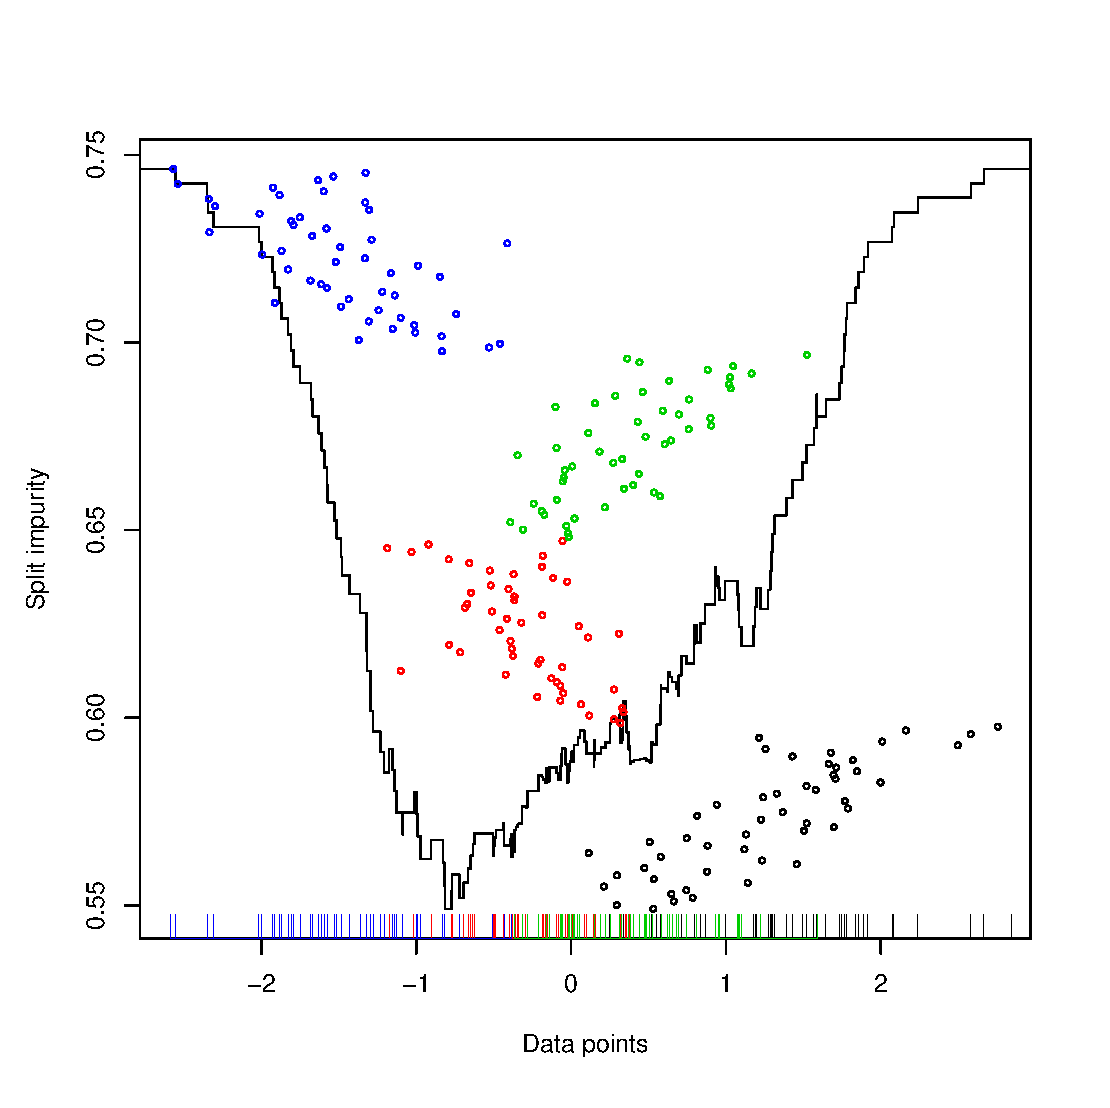
\includegraphics[width=.49\textwidth]{impurity_plot_1d_crabs_data_pc2.ps}
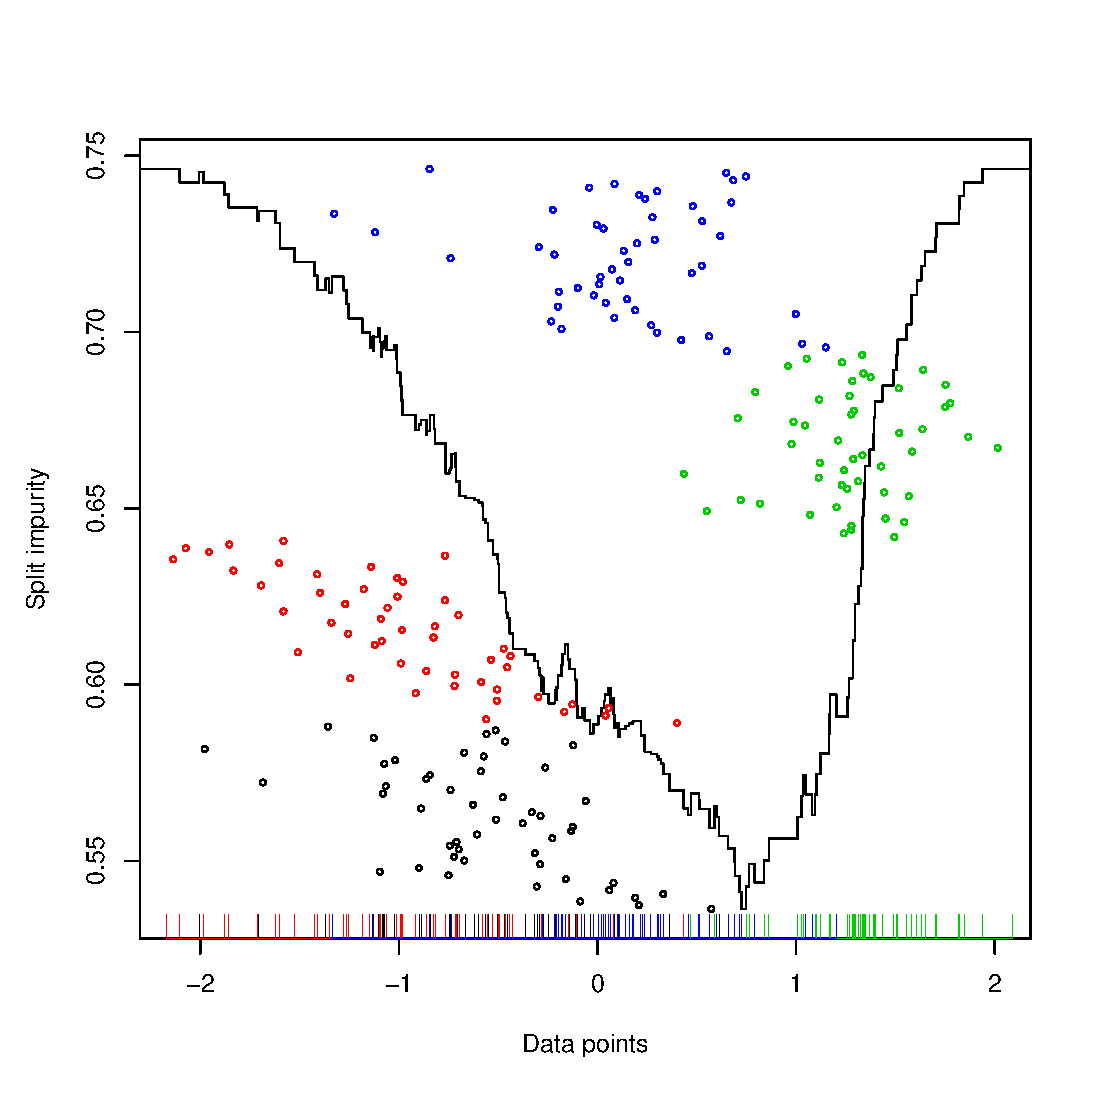
\includegraphics[width=.49\textwidth]{impurity_plot_1d_crabs_data_pc3.ps}
\caption{Plot showing smooth evolution of impurity measure over splits in the axis-parallel split dictionary}
\label{fig:impurity_plot_1d}
\end{figure}

For an arbitrary oblique split $\sum_{i=1}^q a_i X_i=c$, there is much greater freedom to produce similar splits. Increasing (or decreasing) any of the $q$ coefficients results in similar splits (failing to hold only in the unlikely event that many observations take the same value over \emph{all} $q$ continuous attributes). Though these $2^q$ similar splits need not produce unique outcomes, there are still anything between $2\leq m \leq 2^q$ similar outcomes to any given oblique split. Figure~\ref{fig:impurity_plot_2d} shows a typical evolution of the impurity measure when $q=2$.\\

\begin{figure}
\centering
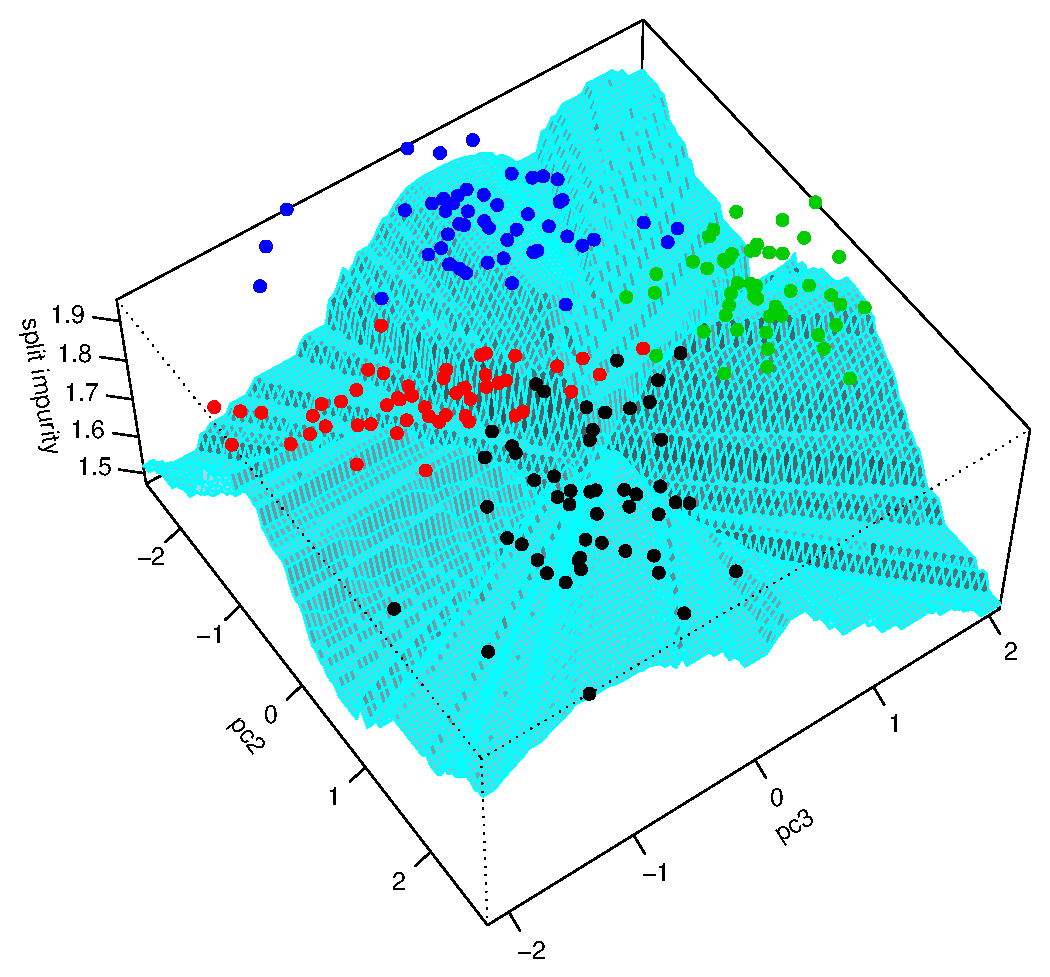
\includegraphics[width=.99\textwidth]{impurity_plot_2d_crabs_data_detail_100_bb.ps}
\caption{Plot showing smooth evolution of impurity surface over sampled splits from the oblique split dictionary}
\label{fig:impurity_plot_2d}
\end{figure}

As considering similar splits only yields marginal information about the impurity surface, it is desireable to avoid similar splits. As the impurity plots show, if observations of different classes lie in contiguous portions of the feature space, split impurity is low in areas \emph{between} these contiguous clusters of observations. For 1-dimensional plots in Figure~\ref{fig:impurity_plot_1d}, it is evident upon closer examination that kinks in the impurity measure occur where class clusters terminate. This phenomenon is particularly evident in Figure~\ref{fig:impurity_plot_2d}, where two valleys are formed which coincide in regions between class clusters. \\

By focusing on regions between class clusters, one can find splits with low impurity values. It is these regions that oblique splits identified in Section~\ref{IdealOutcomes} focus upon.
%Where contiguous structure is present in training data, the set of oblique splits mentioned in Section~\ref{IdealOutcomes} should naturally converge towards these points of interest due to the way in they are defined. 

%By only considering oblique splits that are derived from these ideal splits, not only do we have a much smaller set of splits to evaluate, each evaluated split should reveals a great deal about the impurity surface and such splits should be near to areas with relatively low values of impurity.\\

\begin{comment}
\section{Non-Contiguous and Non-Spherical Class Data}
\label{NonContiguousandNonSphericalClassData}
An obvious question that pops to mind when considering this heuristic argument is the following. When would the subset of oblique splits considered \emph{not} contain split with relatively low values of impurity? Where data is non-contiguous and where one wraps around the other!
\end{comment}

